  \begin{ledgroupsized}[r]{120mm}
                \footnotesize 
                \pstart                
                \noindent\textbf{\"{U}berlieferung:}   
                \pend
                \end{ledgroupsized}
            
              
                           \begin{ledgroupsized}[r]{114mm}
 \footnotesize 
 \pstart \parindent -6mm
\makebox[6mm][l]{\textit{L}}%
Aufzeichnung: LH XXXV 14, 2 Bl. 51. 1 Bl. 8\textsuperscript{o}. 1 S. auf Bl. 51~r\textsuperscript{o}.
Bl.~51~v\textsuperscript{o} überliefert nur 2 Z. von Schreiberhand mit einer \"{U}berschrift aus den \textit{Digesta Iustiniani}, lib. VII, cap. 5:
\textit{Tit. V. De usufructu earum rerum quae usu consumuntur vel minuuntur.}\\%
Cc 2, Nr. 00.
\pend
 \end{ledgroupsized}
 %\normalsize
 \vspace*{5mm}
 \begin{ledgroup}
 \footnotesize 
 \pstart
\noindent%
\footnotesize{\textbf{Datierungsgr\"{u}nde:}
Die \"{U}berschrift auf der R\"{u}ckseite legt die Vermutung nahe, dass es sich beim Textträger des vorliegenden Stücks um Papier für das \title{Corpus juris reconcinnatum} handelt (siehe hierzu \textit{LSB} VI, 2, S. XXIf.). Das St\"{u}ck d\"{u}rfte daher in der Mainzer Zeit nach Beginn der Arbeiten am \textit{CJR} entstanden sein. Eine spätere Datierung ist jedoch nicht ausgeschlossen.}
\pend
 \end{ledgroup}

\vspace*{8mm}
\count\Bfootins=1200
\pstart 
\normalsize
\noindent[51~r\textsuperscript{o}] Concursus Gravitatis duplicis \edtext{unius}{\lemma{duplicis}\Bfootnote{\textit{(1)}\ tum \textit{(2)}\ unius \textit{L }\ }} Liberae\protect\index{Sachverzeichnis}{libra}, alterius in plano inclinato experimentum capi potest. Si grave\protect\index{Sachverzeichnis}{grave} sit liquidum, ut gutta aquae aut cerae\protect\index{Sachverzeichnis}{cera} liquefactae in plani inclinati\protect\index{Sachverzeichnis}{planum inclinatum} superficie inferiore decurrens. Id est non in \textit{a.} sed in \textit{b.} \edtext{Sume}{\lemma{$b.$}\Bfootnote{\textit{(1)}\ ita enim \textit{(2)}\ Sume \textit{L}\ }} candelam\protect\index{Sachverzeichnis}{candela} ardentem hanc oblique tene et observa \edtext{quanta}{\lemma{observa}\Bfootnote{\textit{(1)}\ quousque \textit{(2)}\ quanta \textit{L }}} maxima obliquitate defluat gutta potius in candela,
\begin{window}[0,r,\hspace{2mm}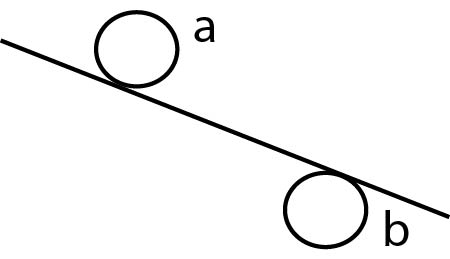
\includegraphics[%trim = -3mm -2mm 0mm 0mm, clip,
width=0.25\textwidth]
{images/lh0351402_51-d.pdf}, \hspace{12mm}{[\textit{Fig. 1}] \vspace{0mm}}]
\noindent
quam delabatur in pavimentum. Fateor tamen gravitatem\protect\index{Sachverzeichnis}{gravitas} tenacitate\protect\index{Sachverzeichnis}{tenacitas} massae\protect\index{Sachverzeichnis}{massa} {adjuvari\reversemarginpar\marginnote{\scriptsize\hspace{-13mm}15}}, sed etsi massa utcunque liquida sit ut in gutta aquae aut Mercurij\protect\index{Sachverzeichnis}{mercurium} aliquamdiu tamen etiam ex plano horizonti parallelo pendere constat, ut in tabulis planis laevigatis sibi impositis fieri videmus. Caeterum hoc experimento aestimari possunt tenacitatis gradus.
\end{window}
%\begin{wrapfigure}[8]{l}{0.25\textwidth}                    
%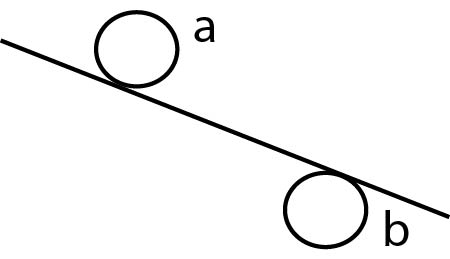
\includegraphics[width=0.25\textwidth]{images/lh0351402_51-d.pdf}\\
%\rule[0cm]{14mm}{0cm}\textit{Fig. 1}\\                       
%%\caption{Bildbeschreibung}
%\end{wrapfigure}
\pend
\pstart Novum \setline{20}cristallisationis\protect\index{Sachverzeichnis}{cristallisatio} genus si aquam in qua sal aliquod solutum \edtext{spissiorem}{\lemma{solutum}\Bfootnote{\textit{(1)}\ est \textit{(2)}\ spissiorem \textit{L}\ }} reddas \edtext{non decoctione,}{\lemma{}\Bfootnote{non\ \textbar\ aquae \textit{gestr.}\ \textbar\ decoctione, \textit{L}}} sed compressione. Ita enim spes est cristallos\protect\index{Sachverzeichnis}{cristallus} nihilo minus micaturas. \pend 
\count\Bfootins=1500


 


